\chapter{本提案手法の機能}\label{cha:Function}
本章では、本研究で提案する帳票画像内の記入欄を自動検出する手法の機能について説明する。

本研究では、帳票画像内の記入欄である領域の座標を取得後、文字の属性を判定し、取得文字近傍に存在する記入欄の座標に対してラベルを割り当て、領域の座標と、対応するラベルを組とするJSON形式のファイルを出力する手法を提案する。
本提案手法は、\ref{sec:input_images}節で述べた帳票画像を入力とする。
出力は、領域の座標と、対応するラベルを組とするJSON(JavaScript Object Notation)形式のファイルと、領域の座標を帳票画像に描画したPNG(Portable Network Graphics)形式の画像である。
出力する画像については、矩形の領域を描画した画像と、下線部の領域を描画した画像の2枚に分けている。
これは、領域の誤検出によって、矩形の領域と下線部の領域が重なった場合、描画した領域が重なることで見づらくなることを防ぐためである。
なお、本研究において、以下の名称を用いる。

\begin{itemize}
    \item 帳票画像記入欄
          入力である帳票画像内の記入欄。
    \item 電子フォーム記入欄
          本提案手法によって取得した座標で示す記入欄。
    \item 領域座標
          本提案手法によって取得した領域の座標。矩形の領域であれば、各頂点のxy座標にあたり、下線部の領域であれば、両端点のxy座標にあたる。
    \item 属性
          文字認識によって得た文字から推測するデータ型。
    \item ラベル
          文字の近傍に存在する電子フォーム記入欄に対して、文字位置と属性から推測するデータ型。
\end{itemize}

また、本研究で提案する手法は、以下の2つの機能を持つ。

\begin{itemize}
    \item ラベル付き領域座標取得機能
    \item 領域描画画像出力機能
\end{itemize}

本提案手法の入力対象である帳票画像を例として、図\ref{fig:original}に示す。
また、図\ref{fig:original}に対して、本提案手法を適用し、出力したJSON形式のファイルの一部を、図\ref{fig:example_output_json}に示す。
出力するJSON形式のファイルの構造を以下に示す。

\begin{itemize}
    \item 矩形領域のラベルと領域の座標をまとめたrects\_dataオブジェクトと、下線部領域のラベルと領域座標をまとめたunderlines\_dataオブジェクトがある。
    \item rects\_dataオブジェクトは、以下のキーとオブジェクトから構成する。
        \begin{itemize}
            \item 取得した矩形の領域座標のうち、どの領域座標かを一意に定める番号を示す、idキー
            \item 領域座標に割り付けたラベルを示す、labelキー
            \item 矩形の領域座標をまとめた、coordsオブジェクト
        \end{itemize}
    \item rects\_dataオブジェクトのcoordsオブジェクトは、以下のオブジェクトから構成する。
        \begin{itemize}
            \item 左上頂点のxy座標をもち、xキーとyキーにそれぞれx座標とy座標が対応するtop\_leftオブジェクト。
            \item 左上頂点のxy座標をもち、xキーとyキーにそれぞれx座標とy座標が対応するbottom\_leftオブジェクト。
            \item 右下頂点のxy座標をもち、xキーとyキーにそれぞれx座標とy座標が対応するbottom\_rightオブジェクト。
            \item 右上頂点のxy座標をもち、xキーとyキーにそれぞれx座標とy座標が対応するtop\_rightオブジェクト。
        \end{itemize}
    \item underlines\_dataオブジェクトは、以下のキーとオブジェクトから構成する。
        \begin{itemize}
            \item 取得した下線部の領域座標のうち、どの領域座標かを一意に定める番号を示す、idキー
            \item 領域座標に割り付けたラベルを示す、labelキー
            \item 下線部の領域座標をまとめた、coordsオブジェクト
        \end{itemize}
    \item underlines\_dataオブジェクトのcoordsオブジェクトは、以下のオブジェクトから構成する。
    \begin{itemize}
        \item 左端点のxy座標をもち、xキーとyキーにそれぞれx座標とy座標が対応するleftオブジェクト。
        \item 右端点のxy座標をもち、xキーとyキーにそれぞれx座標とy座標が対応するrightオブジェクト。
    \end{itemize}
\end{itemize}


\begin{figure}[t]
    \begin{center}
        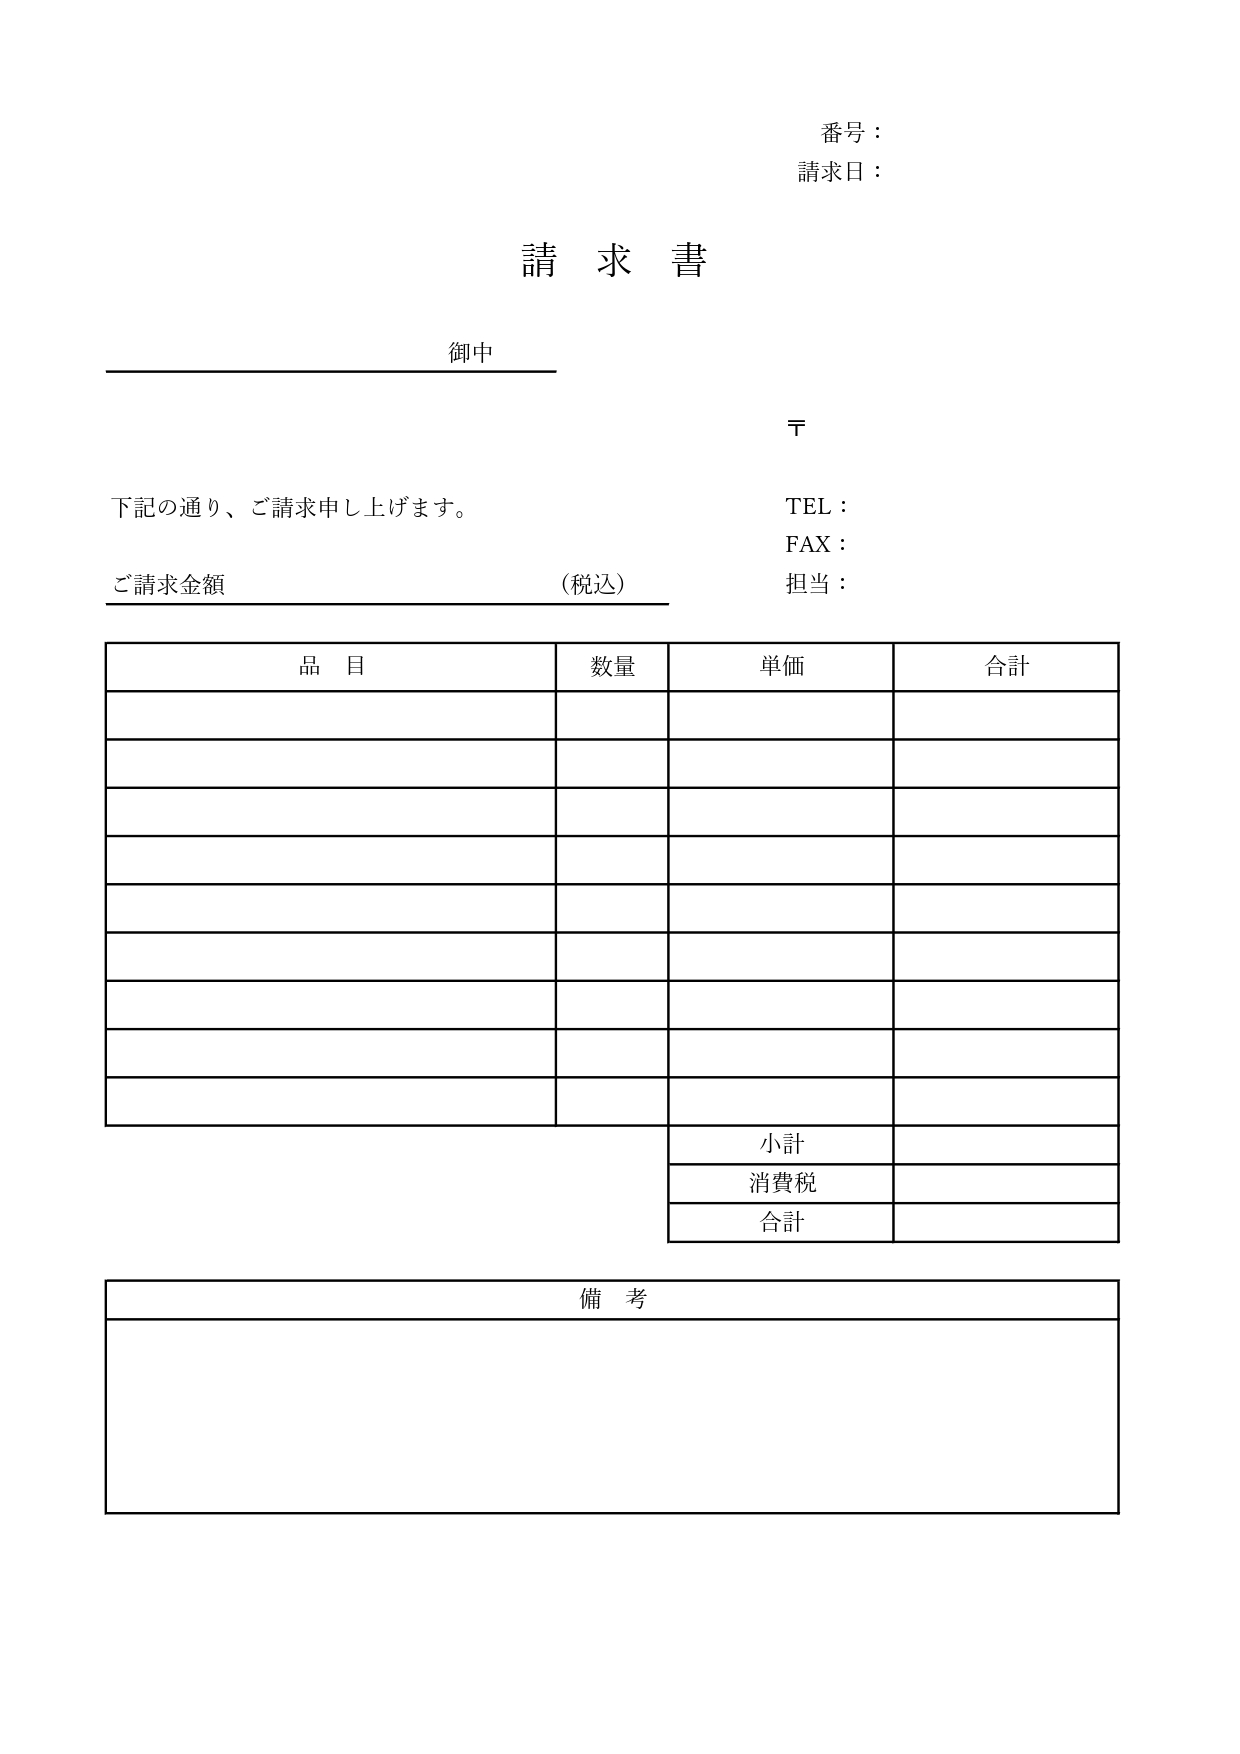
\includegraphics[width=15cm]{image/03-function/original.jpg}
        \caption{元画像}
        \label{fig:original}
    \end{center}
\end{figure}


\lstset{language=}
\begin{figure}[t]
    \begin{lstlisting}
{
    "rects_data": {
        "id": 0, 
        "label": "date",
        "coords": {
            "top_left": {
                "x": 2075,
                "y": 752
            },
            "buttom_left": {
                "x": 2079,
                "y": 953
            },
            "buttom_right": {
                "x": 2190,
                "y": 951
            },
            "top_right": {
                "x": 2186,
                "y": 750
            }
        }
    },
    "underlines_data": {
        "id": 0,
        "label": "string",
        "coords": {
            "left": {
                "x": 213,
                "y": 742
                },
            "right": {
                "x": 1111,
                "y": 742
            }
        }
    }
}
    \end{lstlisting}
    \caption{出力するJSON形式のファイルの一部}\label{fig:example_output_json}
\end{figure}

\begin{figure}[t]
    \begin{center}
        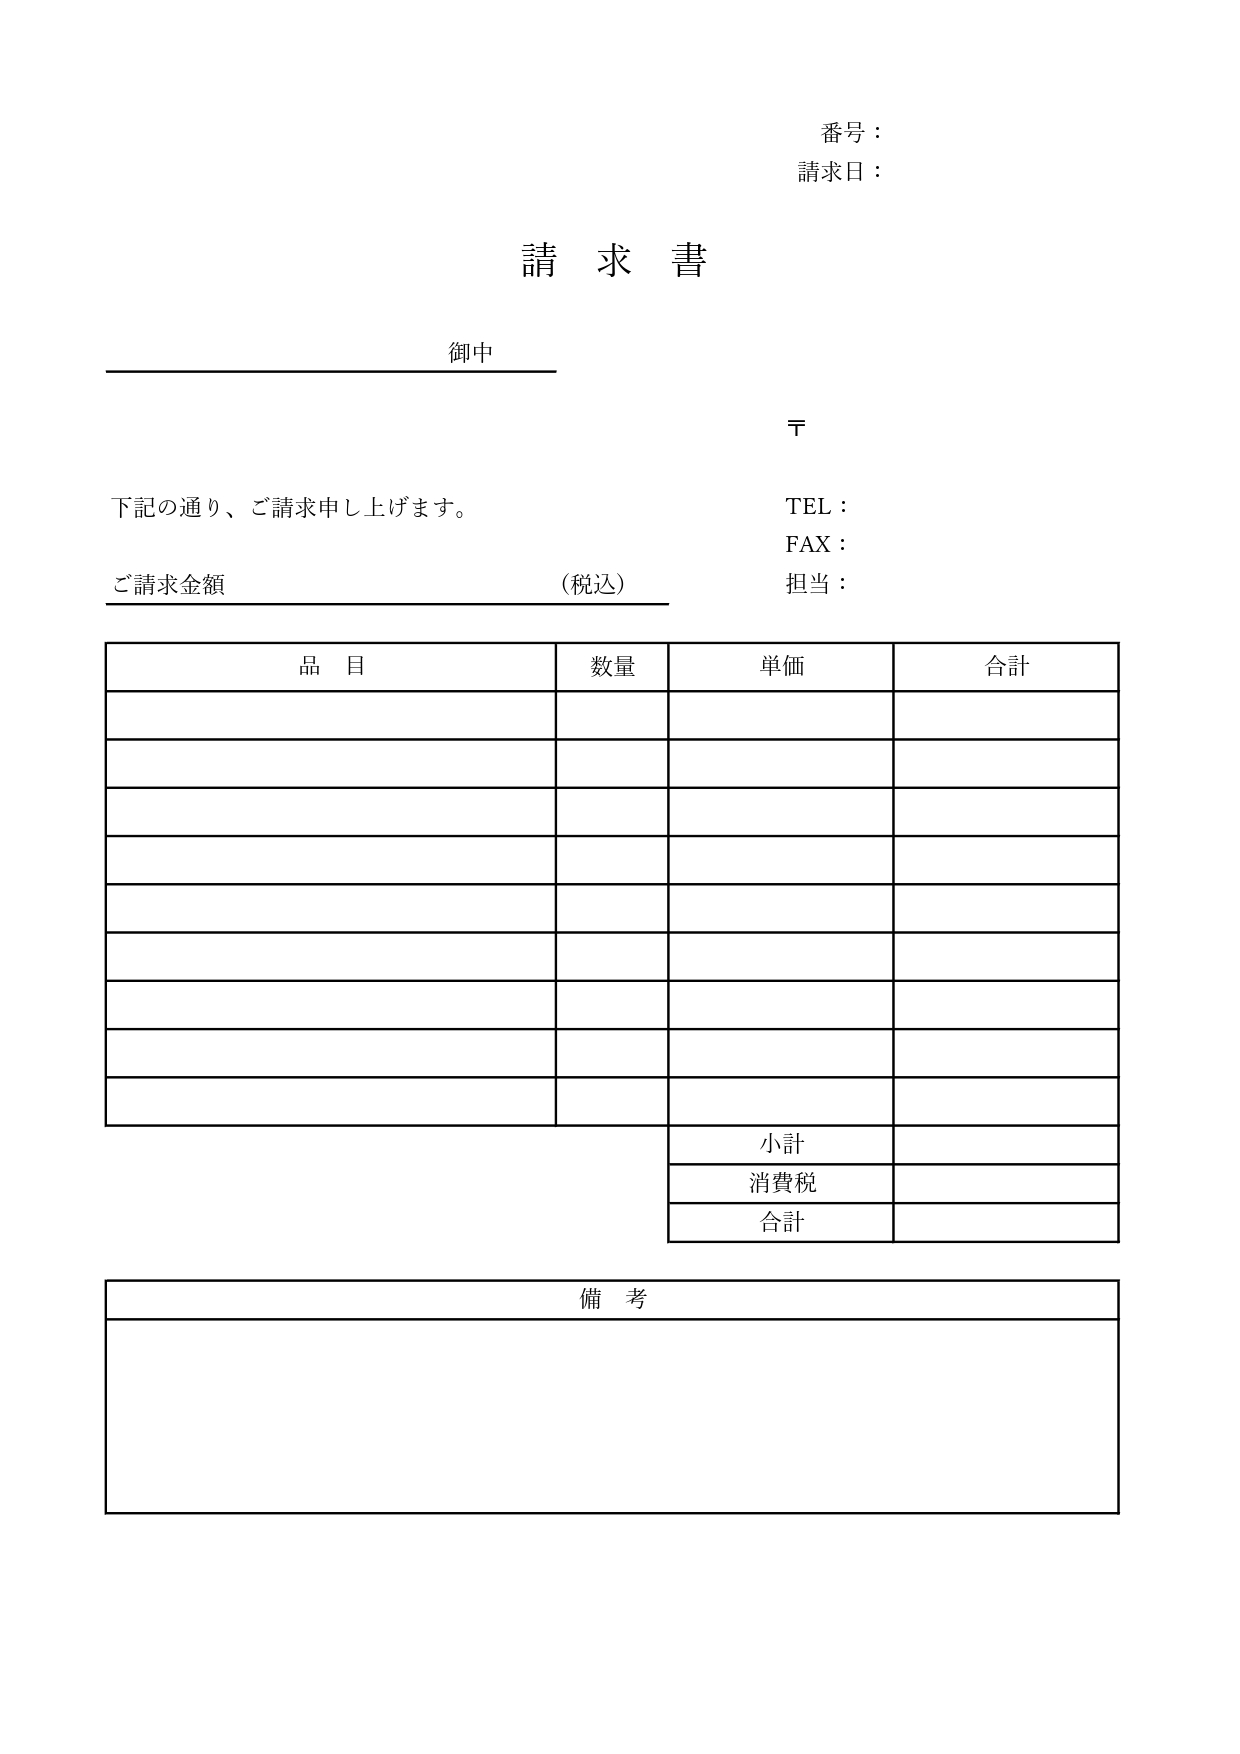
\includegraphics[width=15cm]{image/03-function/original.jpg}
        \caption{元画像}
        \label{fig:original}
    \end{center}
\end{figure}


\section{ラベル付き領域座標取得機能}\label{sec:eform_write_space_obtainment_feature}
ラベル付き領域座標取得機能では、取得対象の記入欄である矩形の領域および下線部の領域について、各領域の座標を電子フォーム記入欄として取得する。

電子フォーム記入欄の取得は、以下の手順で行う。

\begin{enumerate}
    \item 矩形領域取得
    \item 下線部領域取得
    \item 文字および文字位置取得
    \item 属性推測
    \item ラベル割付
\end{enumerate}

\subsection{矩形領域取得}\label{subsec:rect_coords_obtainment}
矩形領域取得は、矩形の領域を帳票画像記入欄とみなし、各頂点のxy座標を領域座標として取得する。
取得した領域座標を、y座標について降順にソートし、0から番号を割り振る。
出力するJSON形式のファイルにおける、rects\_dataオブジェクト内の、idキーに対応する値とcoordsオブジェクトにのデータを取得する。


\subsection{下線部領域取得}\label{subsec:underline_coords_obtainment}
下線部領域取得は、水平な直線上の領域を帳票画像記入欄とみなし、両端点のxy座標を領域座標として取得する。
取得した領域座標を、y座標について降順にソートし、0から番号を割り振る。
出力するJSON形式のファイルにおける、underlines\_dataオブジェクト内の、idキーに対応する値とcoordsオブジェクトのデータを取得する。


\subsection{文字とおよび文字位置の取得}\label{subsec:char_and_bbox_obtainment}
入力である帳票画像に対して文字認識を行い、検出した文字と、検出した文字を囲むバウンディングボックスの各頂点の座標をそれぞれ取得文字、文字位置として取得する。
取得文字と文字位置は、属性推測(\ref{subsec:att_prediction}節で後述)で用いる。

\subsection{属性推測}\label{subsec:att_prediction}
取得文字に対して、大規模言語モデルによる属性の推測を行う。
以下に、属性の候補を定義する。

\begin{itemize}
    \item 日付(date)
    \item 文字列(string)
    \item 数値(number)
\end{itemize}

以上の属性の候補から、取得文字の属性がいずれに該当するかを推測し、属性として取得する。
取得した属性は、ラベル割付(\ref{subsec:label_link}節で後述)で用いる。

\subsection{ラベル割付}\label{subsec:label_link}
\ref{sec:eform_write_space_obtainment_feature}節で得た領域座標と、\ref{subsec:char_and_bbox_obtainment}節で得た文字位置、\ref{subsec:att_prediction}節で得た属性を用いる。
文字位置の近傍に存在する領域座標を対象に属性を割り付け、ラベルとして得る。
出力するJSON形式のファイルにおける、rects\_dataオブジェクト、およびunderlines\_dataオブジェクト内の、labelキーに対応する値を取得する。

ラベル割付後、領域座標と、領域座標に対応するラベルを組としたJSON形式のファイルを、本機能の出力とする。


\section{領域強調画像出力機能}\label{sec:highlighted_area_image_output}
領域強調画像出力機能は、ラベル付き領域座標取得機能(\ref{sec:eform_write_space_obtainment_feature}節)で出力したJSON形式のファイルの内容を、人間の目視で確認しやすくするため、入力である帳票画像に対して、取得した領域座標とラベルを描画し、強調表示した画像を出力する機能である。

図\ref{fig:original}内にある帳票画像記入欄のうち、矩形の帳票画像記入欄の一部を切り取った画像を、図\ref{fig:rect_original}に示す。
また、図\ref{fig:rect_original}の元画像に対し、矩形の領域座標を取得し、描画した画像を、図\ref{fig:rect_drawing}に示す。
図\ref{fig:rect_drawing}の画像内で、矩形領域座標を参照してランダムなRGBカラーで矩形を描画し、同色で矩形左上隅に番号と文字列を表示している。
図\ref{fig:rect_drawing}の矩形に表示する番号は、JSON形式のファイル内のrect\_dataオブジェクトのidキーに対応する値と一致する。
同様に、番号の右に表示する文字列は、JSON形式のファイル内のrects\_dataオブジェクトのlabelキーに対応する値と一致する。

\begin{figure}[t]
    \begin{center}
        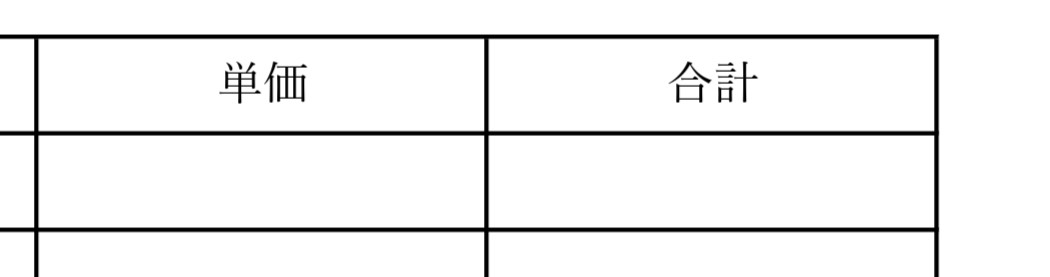
\includegraphics[width=15cm]{image/03-function/rect_original.jpg}
        \caption{帳票画像にある矩形の記入欄}
        \label{fig:rect_original}
    \end{center}
\end{figure}

\begin{figure}[t]
    \begin{center}
        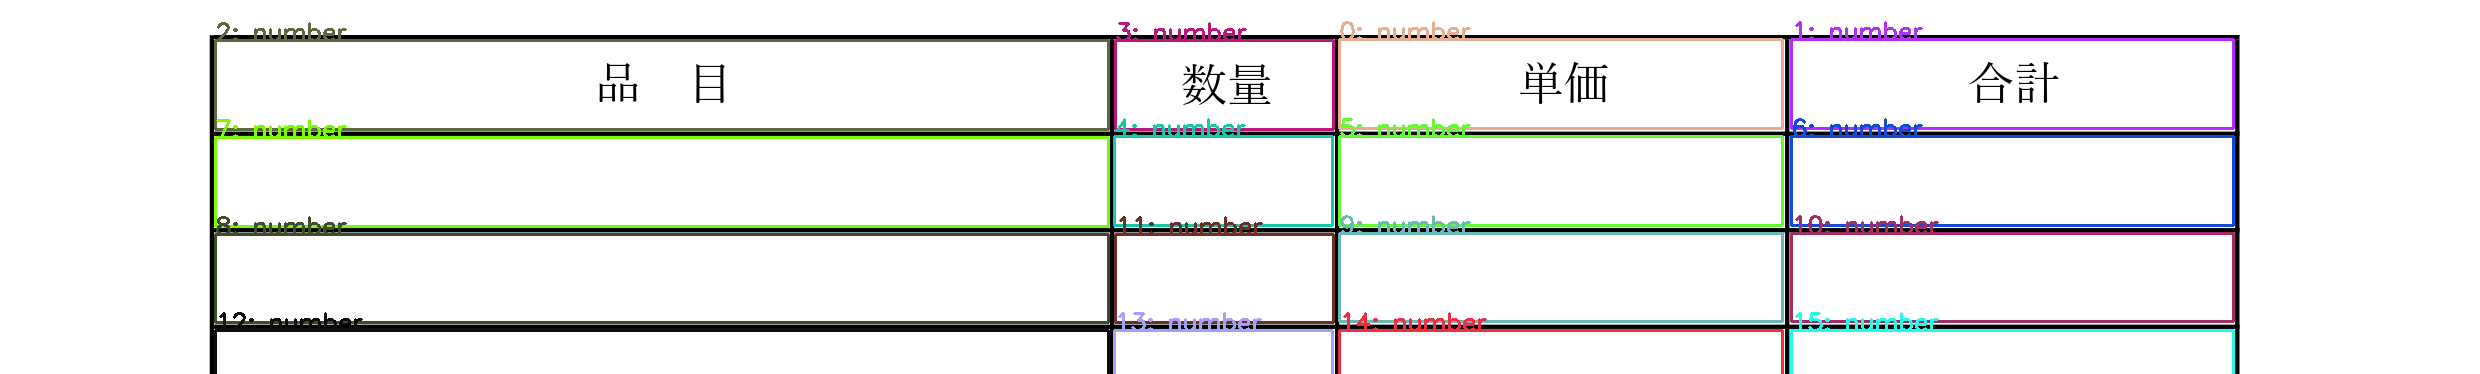
\includegraphics[width=15cm]{image/03-function/rects_with_label.png}
        \caption{取得した矩形領域座標の描画}
        \label{fig:rect_drawing}
    \end{center}
\end{figure}

図\ref{fig:original}内にある帳票画像記入欄のうち、下線部の帳票画像記入欄を切り取った画像を、図\ref{fig:underline_original}に示す。
また、図\ref{fig:underline_original}の画像に対し、下線部の領域座標とラベルを取得し、描画した画像を、図\ref{fig:underline_drawing}に示す。
図\ref{fig:underline_drawing}の画像内で、下線部の領域座標を参照して緑色で直線を描画し、同色で直線の左端点上に番号と文字列を表示している。
図\ref{fig:underline_drawing}の下線部に表示する番号は、JSON形式のファイル内のunderlines\_dataオブジェクトのidキーに対応する値と一致する。
同様に、番号の右に表示する文字列は、JSON形式のファイル内のunderlines\_dataオブジェクトのlabelキーに対応する値と一致する。

\begin{figure}[t]
    \begin{center}
        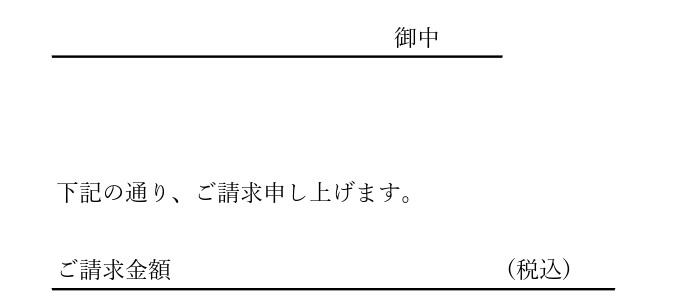
\includegraphics[width=15cm]{image/03-function/underline_original.jpg}
        \caption{帳票画像にある下線部の記入欄}
        \label{fig:underline_original}
    \end{center}
\end{figure}

\begin{figure}[t]
    \begin{center}
        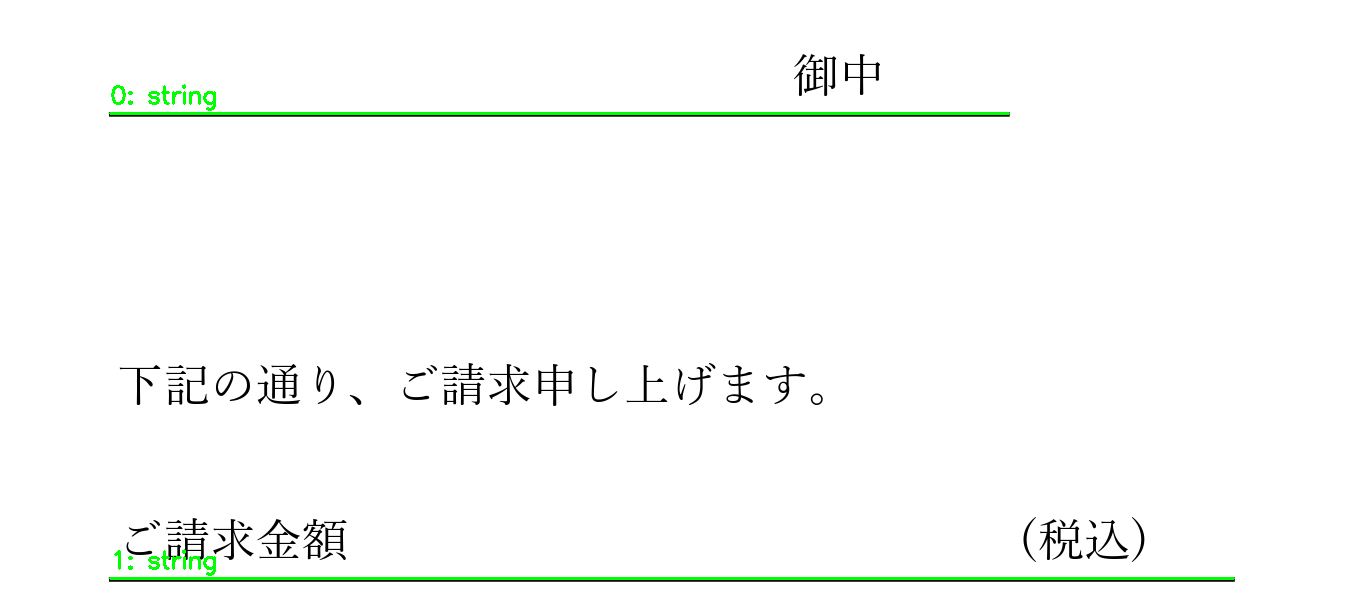
\includegraphics[width=15cm]{image/03-function/underlines_with_label.png}
        \caption{取得した下線部領域座標の描画}
        \label{fig:underline_drawing}
    \end{center}
\end{figure}

図\ref{fig:rect_drawing}、図\ref{fig:underline_drawing}のように、入力である帳票画像に対して、領域座標を描画した画像を本機能の出力とする。

ラベル割付(\ref{subsec:label_link}節)で出力するJSON形式のファイルと、(\ref{sec:highlighted_area_image_output}節)で出力するPNG形式の画像を
